\documentclass[a4paper]{article}

\usepackage[english]{babel}
\usepackage[utf8x]{inputenc}
\usepackage[T1]{fontenc}

\usepackage{graphicx}
\usepackage[colorlinks=true, allcolors=blue]{hyperref}

\title{GIT}
\author{20143750 Kim Subin}

\begin{document}
\maketitle

\section{What is git?}

Git is a distributed version control system to manage program source code. So it doesn't depend on accessing the central server. These days, many developers use git.

\section{Advantages}
It has many advantages. 
\begin{itemize}
	\item First, It is possible to share project folder between users regardless of location. 
    \item Second, It is easy to fetch, merge, branch, and so on. 
    \item Third, It is useful because the processing speed is fast. 		
    \item Last, Open source work becomes easier.
\end{itemize}

\section{How to use git?}
There are two types to use git. The one is git bash, and the other is git gui. If you want to use git, you should know these commands (these 6 commands is basic).
\begin{itemize}
    \item pull : pull the files in remote repository.
    \item push : push the files from local folder to remote repository.
    \item commit : A new commit object is created by saving the workspace or index (stage) source in the local repository. At this point, the pointer pointed to by HEAD and the current branch is changed to the new commit object address. The index pointer also changes to the new commit object address.
    \item merge : Combine two or more development commits.
    \item branch : It means a sort of pruning. If there are developers to proceed a project, they have their own branch, and work in their branch.
    \item checkout : change the branch
\end{itemize}
And this is how to use git bash.
\begin{enumerate}
	\item You can connect to git, create new repository, and copy the git URL.
    \item Enter the folder to put in the remote repository and input "git init" command into your git bash. It means to send it to remote storage.
    \item If you have remote repository already, place the git bash in the desired folder and use command "git clone 'URL' ".
    \item Use the "git add." command, you can add changed files.
    \item "git remote add origin 'address' " It means your local storage connects to the remote storage.
    \item You can push your changed files in local storage to remote storage through this command "git push -u origin master".
    \item If you want to get the files in remote repository, use this command "git pull".
    \item The "branch" is work environment. If you want to check your present branch, use "git branch". 
    \item If you want to change to other branch, use the command "git checkout 'branch name' ".
\end{enumerate}

\section{Github address}
My github address
\url{https://www.github.com/lauren026/assignment01}

\section{Screenshot}

\begin{figure}
\begin{center}
	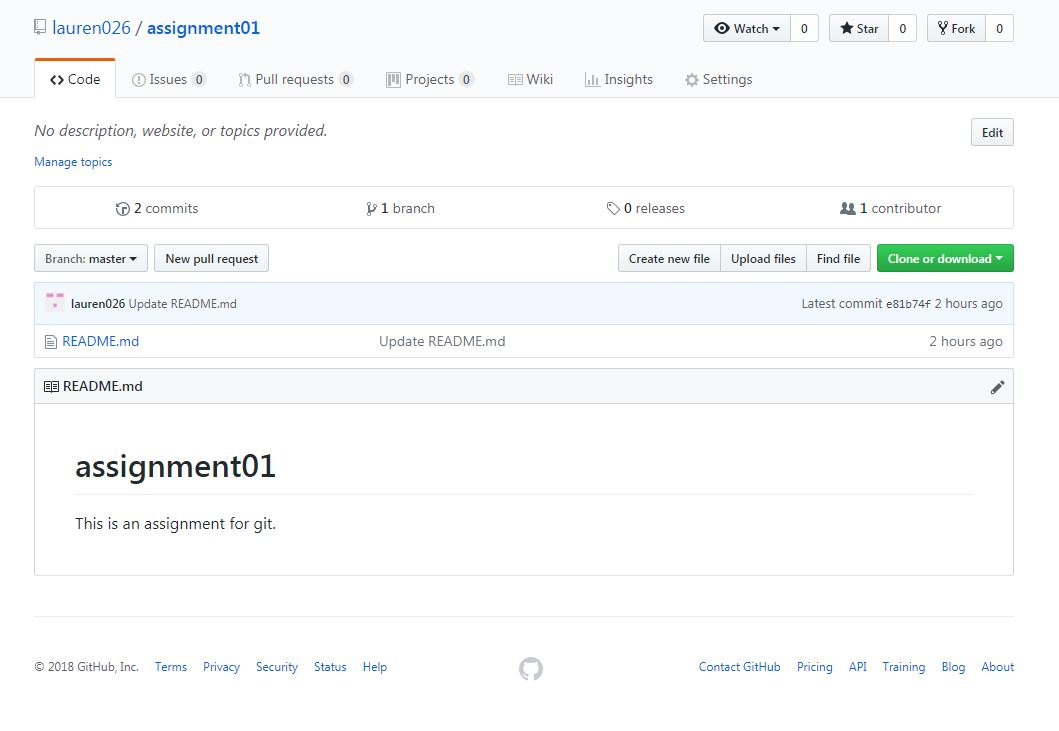
\includegraphics[width=0.8\textwidth]{screenshot01.JPG}
	\caption{\label{fig:screenshot01} This is the original files in my github.}
\end{center}
\end{figure}

\begin{figure}
\begin{center}
	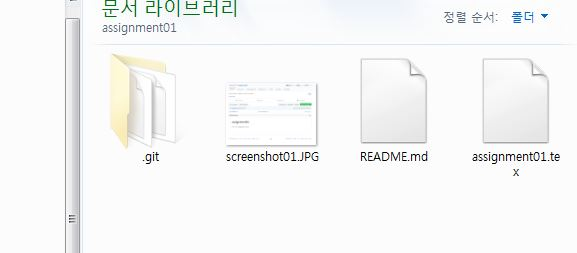
\includegraphics[width=0.8\textwidth]{screenshot02.JPG}
	\caption{\label{fig:screenshot02} I add the modified files to my local folder.}
\end{center}
\end{figure}

\begin{figure}
\begin{center}
	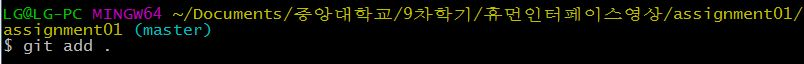
\includegraphics[width=0.8\textwidth]{screenshot03.JPG}
	\caption{\label{fig:screenshot03} "add ." I make list to push files.}
\end{center}
\end{figure}

\begin{figure}
\begin{center}
	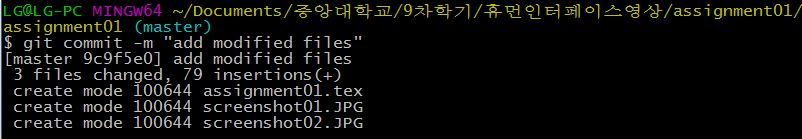
\includegraphics[width=0.8\textwidth]{screenshot04.JPG}
	\caption{\label{fig:screenshot04} I make commit. We can see changed things in figure.}
\end{center}
\end{figure}

\begin{figure}
\begin{center}
	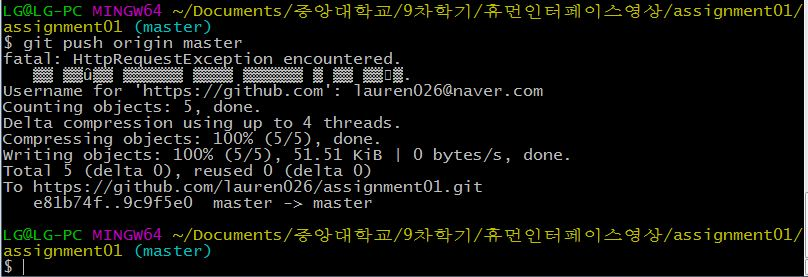
\includegraphics[width=0.8\textwidth]{screenshot05.JPG}
	\caption{\label{fig:screenshot05} "push" I push files to remote repository.}
\end{center}
\end{figure}

\begin{figure}
\begin{center}
	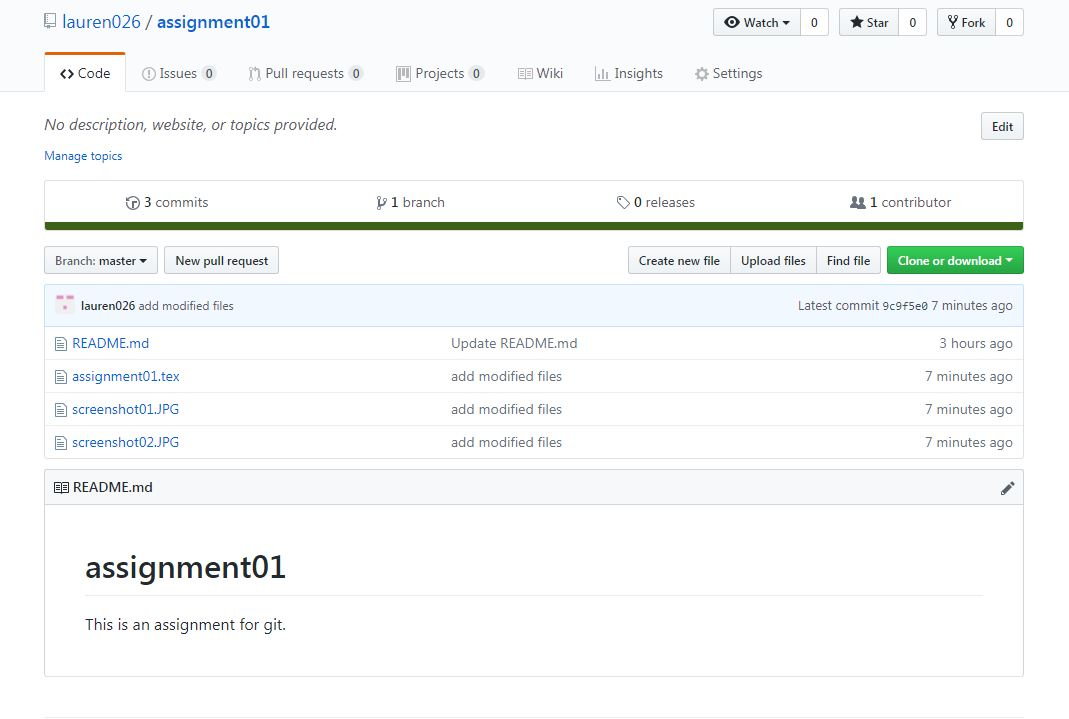
\includegraphics[width=0.8\textwidth]{screenshot06.JPG}
	\caption{\label{fig:screenshot06} Enter the remote repository, github, We can see the modified files in remote repository well.}
\end{center}
\end{figure}

\end{document}